
\section{Hnojiva}
Zvolili jsme kompletní řešení postřiků od fitmy Timac AGRO\footnote{BASF je německá agrochemická firma, která patří k 
největším na světě.\\https://www.agro.basf.cz/agroportal/cz/cs/startpage.html.}.
\footnote{TIMAC AGRO je průmyslovou společností specializující se na pěstování půdy, výživu rostlin a zvířat.\\\url{\detokenize{
https://www.cz.timacagro.com/rostlinna-vyroba/plodinova-doporuceni/repka-olejka.htmll
}}.}.
Pro určení přibližné ceny jednotlivých postřikových přípravků použijeme ceny existujícího polského eshopu https://www.kupnawozy.pl a také
rakouského espohu https://www.samen-schwarzenberger.at. Z obrázku je patrné, že je možné si vybrat z některých produkrů, tedy není nutné použít všechny.
Proto jsme z nich vybrali jen některé. Informace o konkrétních hnojivech jsme vyčetli z oficiálních etiket produktů,
 které je možné nalézt na stránce eagri.cz
\footnote{Vyhledavač:\\\url{\detokenize{
http://eagri.cz/public/app/rhpub/hnojivaVerejnostQF.do
}}. Příklad etikety:\\\url{\detokenize{
http://eagri.cz/public/app/rhpub/etikety/etiketa_36439.pdf?id=36439
}}.}.
\begin{figure}[ht!]
\centering
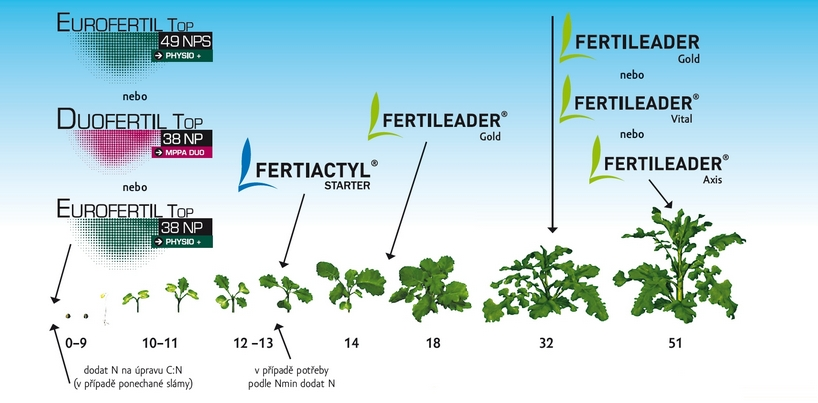
\includegraphics[width=170mm]{img/hnojiva}
\caption{Systém výživy a hnojení řepky ozimé firmy Timac AGRO \label{timac_hnojiva}}
\end{figure}

\subsection{Eurofertil Top 49 NPS}
Obsah látek: (NP 3/22; 24 SO3; 0,15 B; Mescal 975 (29 CaO); Physio+).
\begin{itemize}
  \item Spotřeba 150-250kg/ha.
  \item Cena 2425,0 PLN/t.
\end{itemize}

\subsection{Fertiactyl Starter}
Obsah látek: (13 \% N; 5 \% P2O5; 8 \% K2O; FERTIACTYL® komplex).
\begin{itemize}
  \item Spotřeba kg/ha.
  \item Spotřeba 3l/ha.
  \item Doporučené množství vody 150-500l/ha.
  \item Cena 62,4 PLN/l.
\end{itemize}

\subsection{Fertileader Gold}
Obsah látek: (5,7\%B + 0,35\%Mo + Seactiv).
\begin{itemize}
  \item Spotřeba 3l/ha.
  \item Doporučené množství vody 150-500l/ha.
  \item Cena 16,52 EUR/l.
\end{itemize}

\subsection{Fertileader Vital}
Obsah látek: (9\%N + 5\%P2O5 + 4\%K2O + 0,1\%Mn + 0,05\%B + 0,02\%Cu + 0,02\%Fe + 0,05\%Zn + 0,01\%Mo + Seactiv).
\begin{itemize}
  \item Spotřeba 4l/ha.
  \item Doporučené množství vody 150-500l/ha.
  \item Cena 15,99 EUR/l.
\end{itemize}
